\documentclass{article}
\usepackage[a4paper]{geometry}
\usepackage[english]{babel}
\usepackage[utf8]{inputenc}
\usepackage{url}
\usepackage{hyperref}
\usepackage{graphicx}
\usepackage{amsmath}
\usepackage{amsfonts}
\usepackage{amssymb}
\usepackage{amsthm}
\usepackage{float}

\newcommand{\Sum}[3]{\ensuremath{\displaystyle\sum\limits_{#1}^{#2} #3}}
\newcommand{\scaleFreeFunction}{\ensuremath{p_k = C \cdot k^{-\gamma + 1}}}

\newcommand{\netDescription}[1]{degree distributions in log-log scale of a graph generated using the Barabási-Albert Model with $m_o = 4$, $m = 4$, and #1 nodes. The black points are the data extracted from the graph. The gray dashed line is the curve fit of a power law function \scaleFreeFunction.}

\title{Activity 7}
\author{Lucas Guesser Targino da Silva - RA: 203534}

\begin{document}

\maketitle

\section{Problem Description}

With the help of a computer, generate an undirected network with $N = 10000$ nodes using the Barabasi-Albert model with $m = 4$. Use as initial condition a fully connected network with $4$ nodes.

\begin{enumerate}
    \item Measure the degree distribution at intermediate steps, namely, when the network has 100, 1000, and 10000 nodes.
    \item Compare the cumulative degree distributions at these intermediate steps by plotting them together in a log-log plot and fitting each to a power-law by simple linear regression. Which degrees do you get?  Do they seem to approach the theoretical prediction?
\end{enumerate}

Please hand in your code and figures.

\section{Result}

As stated in \href{http://networksciencebook.com/chapter/5}{Barabasi's book, Chapter 5 on Barabási-Albert Model}, for graph generated with the Barabási-Albert Model, $p_k \propto k^{-3}$ for large values of k.

The Figures \ref{figure:all-100}, \ref{figure:all-1000}, \ref{figure:all-10000}, \ref{figure:large-100}, \ref{figure:large-1000}, \ref{figure:large-10000} were all generated using the data of the graphs and the Cumulative Distribution described in \href{http://networksciencebook.com/chapter/4#advanced-b}{Barabasi's book, Section 4.12, Advanced Topic 3.B: Plotting Power-laws}.

In the Figures \ref{figure:all-100}, \ref{figure:all-1000}, \ref{figure:all-10000}, the exponent of the curve fit is not 3, which may erroneous lead one to believe that the theoretical result ($\gamma = -3$) is wrong. However, as stated in the book, such condition is only valid for ``large values of $k$''. That is exactly what one notices in the Figures \ref{figure:large-100}, \ref{figure:large-1000}, \ref{figure:large-10000} in which the curve fit has been done for $k > 20$.

\textbf{Therefore, the theoretical and experimental results agree.}

\section{Graphs}

\begin{figure}[!ht]
    \centering
    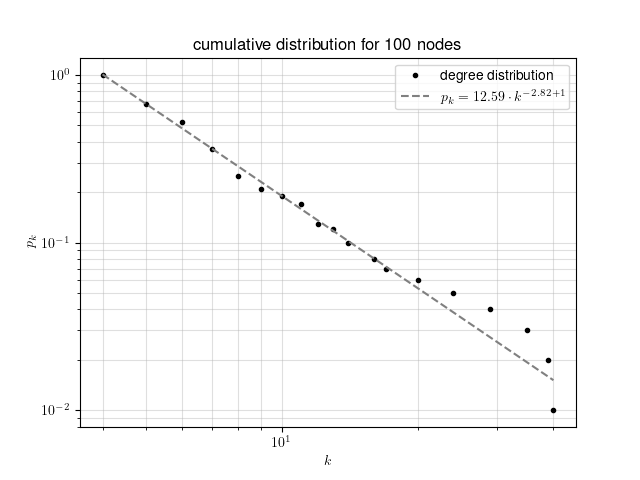
\includegraphics[width=\textwidth]{../result/all_degrees/100.png}
    \caption{\netDescription{100}}
    \label{figure:all-100}
\end{figure}

\begin{figure}[!ht]
    \centering
    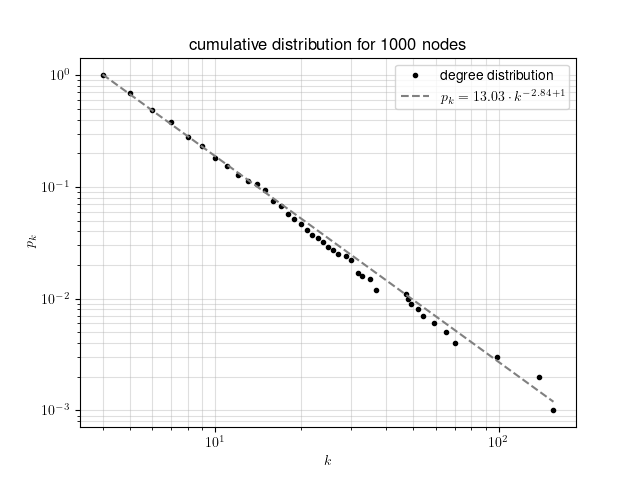
\includegraphics[width=\textwidth]{../result/all_degrees/1000.png}
    \caption{\netDescription{1000}}
    \label{figure:all-1000}
\end{figure}

\begin{figure}[!ht]
    \centering
    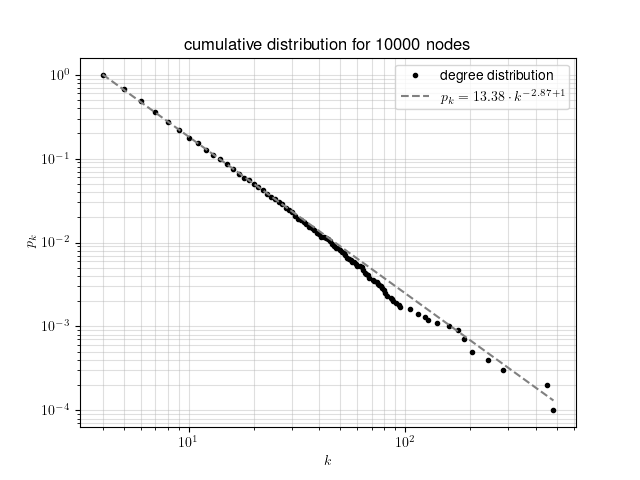
\includegraphics[width=\textwidth]{../result/all_degrees/10000.png}
    \caption{\netDescription{10000}}
    \label{figure:all-10000}
\end{figure}

\begin{figure}[!ht]
    \centering
    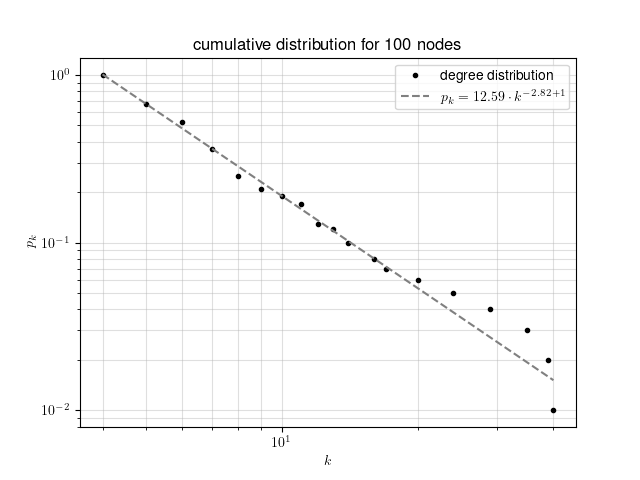
\includegraphics[width=\textwidth]{../result/all_degrees/100.png}
    \caption{\netDescription{100}}
    \label{figure:large-100}
\end{figure}

\begin{figure}[!ht]
    \centering
    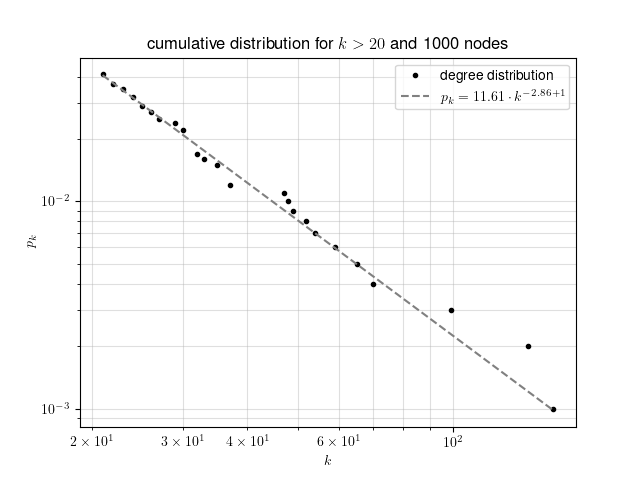
\includegraphics[width=\textwidth]{../result/large_degrees/1000.png}
    \caption{\netDescription{1000}}
    \label{figure:large-1000}
\end{figure}

\begin{figure}[!ht]
    \centering
    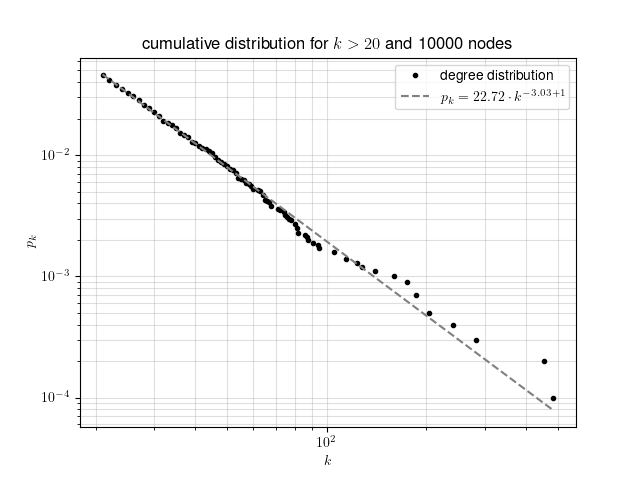
\includegraphics[width=\textwidth]{../result/large_degrees/10000.png}
    \caption{\netDescription{10000}}
    \label{figure:large-10000}
\end{figure}

\end{document}
